\documentclass[a4paper]{article}
\usepackage[english]{babel}
\usepackage[top=1.1cm,headsep=0cm,bottom=1.1cm,footskip=0cm,left=1cm,right=1cm]{geometry}
\usepackage{multicolrule} %다단 본문
\usepackage{fontspec}
	\setmathtt{exprdgs-italic.ttf}[BoldFont = exprdgs-bolditalic.ttf]
\usepackage[colorlinks=true, allcolors=black]{hyperref}
\usepackage{wrapfig} %문단 내 이미지 삽입
\usepackage[abs]{overpic} %이미지 위 텍스트 삽입
\usepackage{graphicx,color} %색상
\usepackage[normalem]{ulem}%취소선
\usepackage{array} %표
\usepackage{mdframed, tcolorbox} %글상자
\usepackage{amsmath, amsfonts, amssymb, bm} %수식

\usepackage[yyyymmdd]{datetime}
\renewcommand{\dateseparator}{-}

	\DeclareMathOperator{\arccsc}{arccsc}
	\DeclareMathOperator{\arcsec}{arcsec}
	\DeclareMathOperator{\arccot}{arccot}
	\DeclareMathOperator{\csch}{csch}
	\DeclareMathOperator{\sech}{sech}
	\DeclareMathOperator{\arcsinh}{arcsinh}
	\DeclareMathOperator{\arccosh}{arccosh}
	\DeclareMathOperator{\arctanh}{arctanh}
	\DeclareMathOperator{\arccsch}{arccsch}
	\DeclareMathOperator{\arcsech}{arcsech}
	\DeclareMathOperator{\arccoth}{arccoth}

	\DeclareMathOperator{\snd}{s}
	\DeclareMathOperator{\meter}{m}
	\DeclareMathOperator{\cm}{cm}
	\DeclareMathOperator{\mm}{mm}
	\DeclareMathOperator{\mum}{\mu m}

	\DeclareMathOperator{\newton}{N}
	\DeclareMathOperator{\kn}{kN}
	\DeclareMathOperator{\kgf}{kgf}

	\DeclareMathOperator{\pa}{Pa}
	\DeclareMathOperator{\kpa}{kPa}
	\DeclareMathOperator{\mpa}{MPa}
	\DeclareMathOperator{\gpa}{GPa}
	\DeclareMathOperator{\mmhg}{mmHg}
	\DeclareMathOperator{\knpm}{kN/m}
	
	\DeclareMathOperator{\mps}{m/s}
	\DeclareMathOperator{\mpss}{m/s^2}
	
	\DeclareMathOperator{\dgr}{\!^\circ}
	\DeclareMathOperator{\cel}{\!^\circ C}
	\DeclareMathOperator{\fer}{\!^\circ F}
	\DeclareMathOperator{\kel}{K}
	
	\DeclareMathOperator{\kg}{kg}
	\DeclareMathOperator{\kgpcm}{kg/m^3}
	\DeclareMathOperator{\cmpkg}{m^3/kg}
	
	\DeclareMathOperator{\nm}{N\cdot m}
	
	\DeclareMathOperator{\watt}{W}
	\DeclareMathOperator{\kw}{kW}
	\DeclareMathOperator{\kwh}{kWh}
	
	\DeclareMathOperator{\joule}{J}
	\DeclareMathOperator{\kj}{kJ}
	\DeclareMathOperator{\jpkg}{J/kg}
	\DeclareMathOperator{\kjpkg}{kJ/kg}
	\DeclareMathOperator{\kjpkk}{kJ/kg\cdot K}
	\DeclareMathOperator{\kps}{kg/s}
	
	\DeclareMathOperator{\satat}{sat\,@}

\usepackage{polynom} %나눗셈 필산
\usepackage{cancel} %수식 약분선
\usepackage{titlesec} %섹션 이름 변경
\usepackage{kotex} %한글
\usepackage{fancyhdr} %페이지 넘버 편집
	\pagestyle{fancy}
	\renewcommand{\headrulewidth}{0pt}
	\fancyhf{}
	\fancyhead[R]{p.\thepage}
	\fancyfoot[R]{\color{red}[\LaTeX]}

\setlength\columnsep{2cm}
\SetMCRule{
	width = 0.3mm,
	color-model = rgb,
	color = {0.9,0.9,0.9},
	line-style = dashed
	}
	
\newcommand{\solution}{\noindent\textbf{[Solution]}}

\renewcommand{\section}[1] {
	\vspace{\baselineskip}
	\noindent\hspace{-1.0cm}\begin{overpic}{qframe.png}
		\put(8mm,-0.3mm){
			\begin{tcolorbox}[
				boxsep = 0mm,
				top = 0mm,
				bottom = 0mm,
				left = 0mm,
				right = 0mm,
				boxrule = 0mm,
				colback = white,
				colframe = blue,
				width = 2.2cm,
				height = 8mm,
				halign = center,
				valign = center,
				sharp corners = all,
				opacityfill = 0,
				fontupper = \bfseries
				]
				{[ #1 ]}
			\end{tcolorbox}
		}
	\end{overpic}
}

\makeatletter
\renewcommand{\maketitle}{\setlength{\parindent}{0pt}
	\begin{flushleft}
		\LARGE{\textbf{\@title}}\\
		\vspace{0.6cm}
		\LARGE{\qquad\@author}
		\vspace{0.5cm}
	\end{flushleft}
	\hspace{-1cm}\noindent\textcolor{red}{\rule{21cm}{0.5mm}}
}
\makeatother

\title{열역학(다)\hspace{7cm} Report \#1}
\author{기계공학부,\qquad 2022****,\qquad 2학년,\qquad ***\qquad\qquad{\normalsize 작성일 : \today}}
\date{}

\begin{document}

\maketitle

\begin{multicols*}{2}

\setlength{\parindent}{3mm}

\noindent
\textbf{\Large{}}\\[5pt]
\textbf{\large{R1 - 1}}\\[5pt]
\textbf{\large{R1 - 2}}\\[5pt]
\textbf{\large{R1 - 3}}\\[5pt]
\textbf{\large{R1 - 4}}\\

\section{R1 - 1}
	\vspace{-\baselineskip}
	\begin{align*}
		&m = 1\kg,\quad\mathtt{V} = 0.15\meter^3 = \text{const.},\\
		&P_1 = 2\mpa,\quad T_2 = 40\cel
	\end{align*}
	(a) Find $T_1$.\\
	(b) Find $P_2$.\\
	(c) Draw a $T$-$\mathtt{v}$ diagram.\\
	
	\solution\\[10pt]
	Before cooling,
	\begin{align*}
		&\mathtt{v} = \frac{\mathtt{V}}{m} = 0.15\cmpkg\\
		&\mathtt{v}_{f@P_1} = \mathtt{v}_{f@2000\kpa} = 0.001177\cmpkg\\
		&\mathtt{v}_{g@P_1} = \mathtt{v}_{g@2000\kpa} = 0.099587\cmpkg\\
		&\mathtt{v} > \mathtt{v}_{g,@P_1} \quad\Rightarrow\quad \text{superheated vapor}
	\end{align*}
	@\;$P = 2\mpa$\quad \begin{tabular}{|c|c|}
		\hline
		$T\,[\,\cel]$ & $\mathtt{v}\,[\cmpkg]$\\
		\hline
		$350$ & $0.13860$\\
		\hline
		$T_1$ & $0.15000$\\
		\hline
		$400$ & $0.15122$\\
		\hline
	\end{tabular}
	\begin{align*}
		&T_1 = \frac{400-350}{0.15122 - 0.13860}(0.15 - 0.13860) + 350\\
		&\quad = 395.1664025 \approx 395.17\cel
	\end{align*}
	After cooling,
	\begin{align*}
		&\mathtt{v}_{f@T_2} = \mathtt{v}_{f@40\cel} = 0.001008\cmpkg\\
		&\mathtt{v}_{g@T_2} = \mathtt{v}_{g@40\cel} = 19.515\cmpkg\\
		&\mathtt{v}_{f@T_2} \leq \mathtt{v} \leq \mathtt{v}_{g@T_2} \quad\Rightarrow\quad \text{wet vapor}\\
		&P_2 = P_{\satat 40\cel} = 7.3851\kpa
	\end{align*}
	\begin{center}
		\includegraphics{img/001.png}
	\end{center}

\section{R1 - 2}
	\vspace{-\baselineskip}
	\begin{align*}
		&T_1 = 300\cel,\quad P = 0.5\mpa = \text{const.},\\
		&m = 0.6\kg,\quad x=0.48
	\end{align*}
	(a) Find $T_2$, $\mathtt{v}_2$, $m_{f2}$.\\
	(b) Determine $\Delta \mathtt{V}$.\\
	(c) Draw a $T$-$\mathtt{v}$ diagram.\\
	
	\solution\\[10pt]
	Before cooling,
	\begin{align*}
		&P_{\satat 300\cel} = 8587.9\kpa > P = 500\kpa\\
		&\Rightarrow \quad \text{superheated vapor}\\
		&\mathtt{v}_1 = \mathtt{v}_{@\,0.5\mpa,300\cel} = 0.52261\cmpkg
	\end{align*}
	After cooling,
	\begin{align*}
		&0<x<1 \quad \Rightarrow \quad \text{wet vapor}\\
		&m_{f2} = m(1-x) = (0.6)(1-0.48) = 0.312000\\
		&\quad \approx 0.3120\kg\\
		&T_2 = T_{\satat 500\kpa} = 151.83\cel\\
		&\mathtt{v}_{f2} = \mathtt{v}_{f@500\kpa} = 0.001093\cmpkg\\
		&\mathtt{v}_{g2} = \mathtt{v}_{g@500\kpa} = 0.37483\cmpkg\\
		&\mathtt{v}_{2} = \mathtt{v}_{f2} + x(\mathtt{v}_{g2} - \mathtt{v}_{f2})\\
		&\quad = 0.001093 + (0.48)(0.37483 - 0.001093)\\
		&\quad = 0.18048676 \approx 0.18049 \cmpkg\\
		&\Delta \mathtt{V} = m(\mathtt{v}_{2} - \mathtt{v}_{1})\\
		&\quad = (0.6)(0.18048676 - 0.52261)\\
		&\quad = -0.205273944 \approx -0.2053\meter^3
	\end{align*}
	\begin{center}
		\includegraphics{img/002.png}
	\end{center}

\section{R1 - 3}
	\vspace{-\baselineskip}
	\begin{align*}
		&P_1 = P_2 = 3.5\mpa\neq P_3,\quad T_2 = T_{\satat 3.5\mpa}\\
		&T_1 = T_2 + 5\cel,\quad T_3 = 200\cel,\quad \mathtt{v}_1 \neq \mathtt{v}_2 = \mathtt{v}_3
	\end{align*}
	\begin{tabular}{ll}
		(a) Find $T_1$. &\qquad (d) Draw a $T$-$\mathtt{v}$ diagram.\\
		(b) Find $\Delta h_{1\to2}$. &\\
		(c) Find $P_3$ and $x_3$.
	\end{tabular}\\

	\solution\\[10pt]
	At the state 1, it is superheated vapor. Therefore,
	\begin{align*}
		&T_1 = T_{\satat 3.5\mpa} + 5\cel = 242.56 + 5 = 247.56000\\
		&\quad \approx 248 \cel
	\end{align*}
	@\;$P = 3.5\mpa$\quad \begin{tabular}{|c|c|}
		\hline
		$T\,[\,\cel]$ & $h\,[\kjpkg]$\\
		\hline
		$242.56$ & $2802.7$\\
		\hline
		$247.56$ & $h_1$\\
		\hline
		$250.00$ & $2829.7$\\
		\hline
	\end{tabular}
	\begin{align*}
		&h_1 = \frac{247.56 - 242.56}{250-242.56}(2829.7 - 2802.7) + 2802.7\\
		&\quad = 2820.845161 \approx 2821\kjpkg
	\end{align*}
	At the state 2, it is saturated liquid water. Therefore,
	\begin{align*}
		&h_2 = h_{f@3.5\mpa} = 1049.7\kjpkg\\
		&\Delta h_{1\to2} = h_2 - h_1 = 1049.7 - 2820.845161\\
		&\quad = -1771.145161 \approx -1771.1/\kjpkg\\
		&\mathtt{v}_2 = \mathtt{v}_{f@3.5\mpa} = 0.001235\cmpkg
	\end{align*}
	At the state 3, it is wet vapor. Therefore,
	\begin{align*}
		&\text{given :}\quad T_3 = 200\cel\\
		&P_3 = P_{\satat 200\cel} = 1554.9\kpa\\
		&\mathtt{v}_3 = \mathtt{v}_2 = 0.001235\cmpkg\\
		&\mathtt{v}_{f3} = \mathtt{v}_{f@200\cel} = 0.001157\cmpkg\\
		&\mathtt{v}_{g3} = \mathtt{v}_{g@200\cel} = 0.12721\cmpkg\\
		&x_3 = \frac{\mathtt{v}_{3} - \mathtt{v}_{f3}}{\mathtt{v}_{g3} - \mathtt{v}_{f3}} = \frac{0.001235 - 0.001157}{0.12721 - 0.001157}\\
		&\quad = 6.187873355\times10^{-4} \approx 0.0619\%
	\end{align*}
	\begin{center}
		\includegraphics{img/003.png}
	\end{center}
	
\section{R1 - 4}
	\vspace{-\baselineskip}
	\begin{align*}
		&T_1 = 20\cel,\quad P_1 = 170\kpa,\quad m_1 = 10\kg\\
		&T_2 = 29\cel,\quad P_2 = 300\kpa,\quad \mathtt{V} = \text{const.},\quad Z =1
	\end{align*}
	Determine $\Delta m$.\\[10pt]
	\solution
	\begin{align*}
		&T_1 = (20 + 273.15)\kel = 293.15\kel\\
		&T_2 = (29 + 273.15)\kel = 302.15\kel\\
		&P\mathtt{V} = mRT \quad\Rightarrow\quad \frac{R}{\mathtt{V}} = \frac{P}{mT} = \text{const.}\\
		&\frac{P_1}{m_1T_1} = \frac{P_2}{m_2T_2} \quad\Rightarrow\quad m_2 = \frac{m_1T_1P_2}{T_2P_1}\\
		&\Delta m = m_2 - m_1 = \frac{m_1T_1P_2}{T_2P_1} - m_1
	\end{align*}
	\begin{align*}
		&\quad = \frac{(10)(293.15)(300)}{(302.15)(170)} - 10 = 7.1214141788\\
		&\quad \approx 7.1214\kg
	\end{align*}



\end{multicols*}
\end{document}